\subsection{Word Classifier and Different Initialization Methods}\label{sec:word_classifier_results}
In this subsection the classification results for running with the words in Table~\ref{tab:words_supported_by_classifier} will be presented. 
The training and test example words were randomly generated with the generator having the properties in Table~\ref{tab:word_generator_properties}.
See Section~\ref{sec:dataset}, for more information about the word example generator. 

We used a total of 100 test examples to test the accuracy of the created classifiers.
Five test examples each for the 20 words. 
The test examples were generated using the same properties as the training examples.
Two initialization methods, count-based initialization and random initialization, were tested with 100, 200, 400, 800 and 1600 training examples. 
The results of the test is presented in Figure~\ref{figure:initialization-methods}. 
It contains the test scores for the two initialization methods, before and after training with the Baum-Welch algorithm. 
The test score is defined as the percentage of correctly classified test examples.

\begin{table}[htb]
  \begin{center}
  \begin{tabular}{ l l l l l }
    dog      & cat       & pig     & love       & hate  \\
    scala    & python    & summer  & winter     & night  \\ 
    daydream & nightmare & animal  & happiness  & sadness \\ 
    tennis   & feminism  & fascism & socialism  & capitalism \\
  \end{tabular}
\end{center}
\caption{Words supported by the resulting classifier.} 
\label{tab:words_supported_by_classifier} 
\end{table}

\begin{table}[htb]
  \begin{center}
  \begin{tabular}{ l l }
    Probability of extra letter at position         & 0.03 \\
    Probability of extra letter equal neighbor      & 0.7 \\ 
    Probability of wrong letter at position         & 0.1 \\ 
    Probability of letter missing at position       & 0.03 \\
  \end{tabular}
\end{center}
\caption{Properties enforced by the word training example generator.} 
\label{tab:word_generator_properties} 
\end{table}

\begin{figure}[h!]
\centering
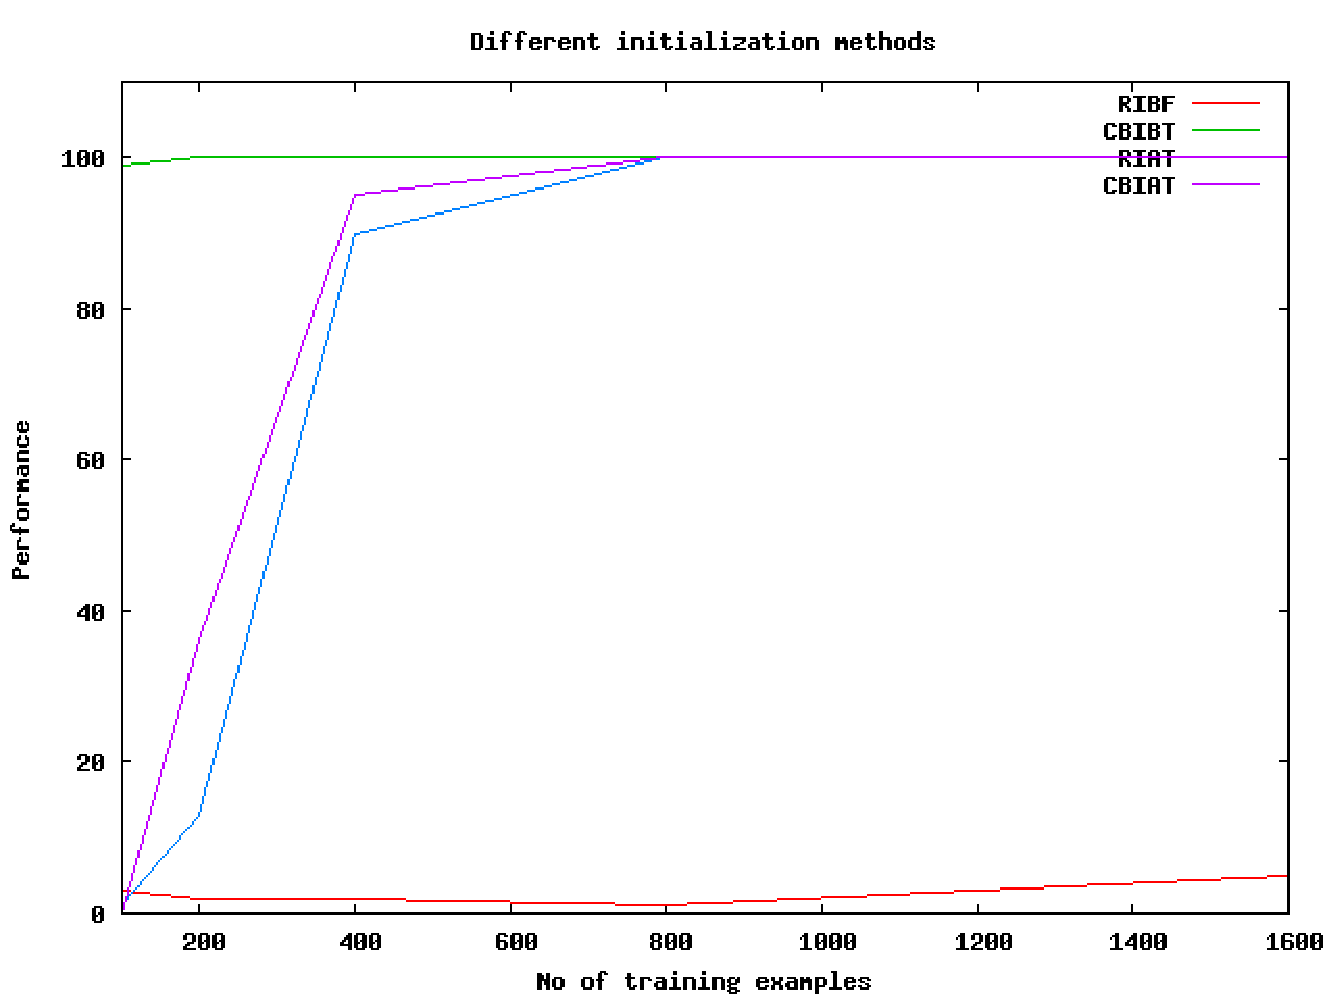
\includegraphics[scale=0.57]{initialization-methods}
\caption{Test with different number of training examples and different initialization methods.
	 NOE=''number of training examples for every word'',
         RIBF=''random initialization score before training'',
         CBIBT=''count-based initialization score before training'',
         RIAT=''random initialization score after training'',
         CBIAT=''count-based initialization score after training.}
\label{figure:initialization-methods}
\end{figure}

\subsection{Test of Single HMM Word Classifier}
\textbf{TODO:} Here results for the word classifier called \textit{Word HMM} in the Topology of Word Classifier Section will be presented.


\subsection{Character Classification with Different Parameters}\label{sec:character_classifier_results}

As described in Section~\ref{sec:image-preprocessing} the image feature extraction step in the character classifier takes two parameters.
The first parameter is the \textit{number of segments} that should be created. 
The second parameter is the \textit{size classification factor}, which is used in Equation~\ref{eq:classification_function}. 
For the experiment we only had 100 examples for each of the 26 characters. 
How the examples are produced is described in Section~\ref{sec:dataset}. 
An initial experiment was performed to test count-based initialization and random initialization before and after training with the Baum-Welch algorithm.
The initial experiment shows that there is probably not enough training data for the training to have any positive effect for count-based initialization. 
This could possible be fixed to some extend with some kind of smoothening of the model produced by the training. 
10 test examples and 90 training examples for every character were selected randomly from the example set for the experiments. 
The results from the initial experiment can be found in table~\ref{tab:character_classifier_initial_experiment}. 
In the initial experiment $1.3$ was used as the size classification factor and the number of segments was set to $7$.


\begin{table}[htb]
  \begin{center}
  \begin{tabular}{ l l l l l }
    NOE    & RIBF   & CBIBT  & RIAT    & CBIAT \\ \hline
    $90$  & $4\%$ & $53\%$ & $16\%$  & $16\%$  \\   
  \end{tabular}
\end{center}
\caption{Test of the character classifier with different initialization methods and before and after training.
	 NOE=''number of training examples for every word'',
         RIBF=''random initialization score before training'',
         CBIBT=''count-based initialization score before training'',
         RIAT=''random initialization score after training'',
         CBIAT=''count-based initialization score after training''} 
\label{tab:character_classifier_initial_experiment} 
\end{table}

Only count-based initialization is considered in the experiment of different parameters, because the initial experiment showed that the best result seems to be produced when only using count-based initialization and no training.
When testing the parameters, 5 models were created in the same way as in the initial experiment. 
The average accuracy for these 5 models when testing them with their own test example set was recorded as the accuracy for the configuration. 
For all 5 models that were created, different training example sets and test example sets were randomly selected. 
We used 90 training examples and 10 test examples for every character, as in the initial experiment. 
The results of the experiment can be seen in Figure~\ref{figure:charater-results-parameters}.

\begin{figure}[h!]
\centering
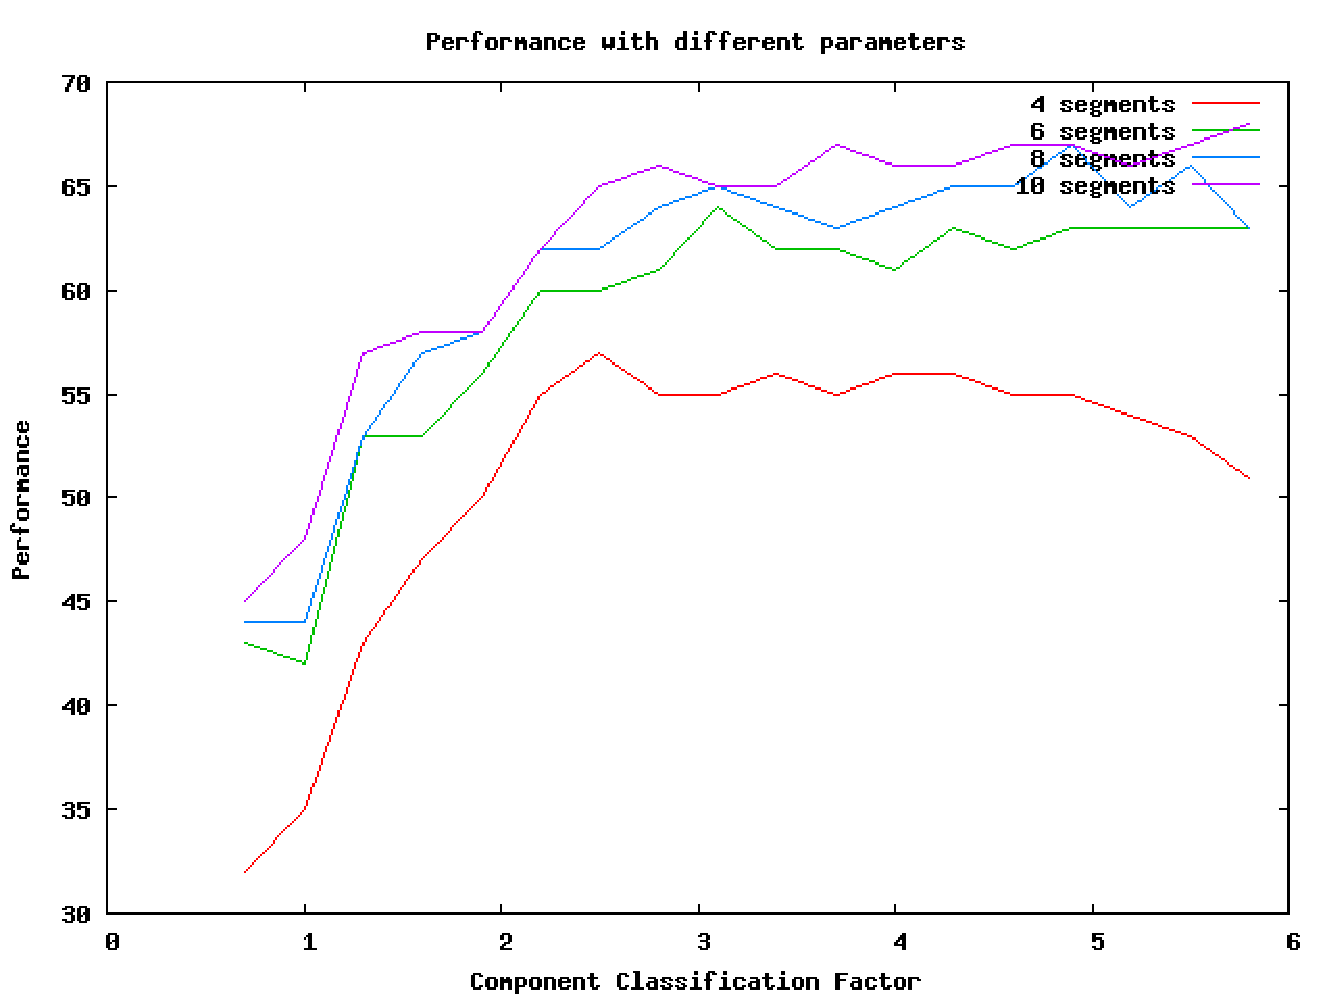
\includegraphics[scale=0.57]{ccf-nos}
\caption{Results for character classification test with different parameters. The performance is the percentage of correctly classified characters.}
\label{figure:charater-results-parameters}
\end{figure}



